\subsection{Modélisation des \awss}

La fonctionnalité des \awss\ annoncée en partie~\ref{section:eyrolles_fct} se résume à permettre à l'application développée, le \alotdeux, de communiquer avec la partie de l'\aintranet\ déjà existante, le \alotun.

Techniquement, un \aws\ est une interface (\aapi) accessible via un réseau et qui permet d'exécuter des actions sur un système distant. Dans le cas d'\aey, c'est le \alotdeux\ qui utilise l'interface du \alotun\footnote{Les \awss\ du \alotun\ sont développés en interne chez \aey.}, et jamais l'inverse. Les \awss\ du \alotdeux\ consistent alors à envoyer des données dans le bon format aux \awss\ du \alotun, et éventuellement de recevoir une réponse. Les données sont échangées via le protocole \ahttp, et le format de données utilisé est le \ajson\footnote{JSON (JavaScript Object Notation) est un format de données textuel permettant de représenter de l'information structurée.\\Exemple : \texttt{\{"auteur": \{"id": "1", "nom": "Jean Dupont"\}\}}}. La figure~\ref{figure:eyrolles_webservices_echange} illustre la façon dont les lots indépendants de l'\aintranet\ d'\aey\ communiquent.

\begin{figure}
	\centering
	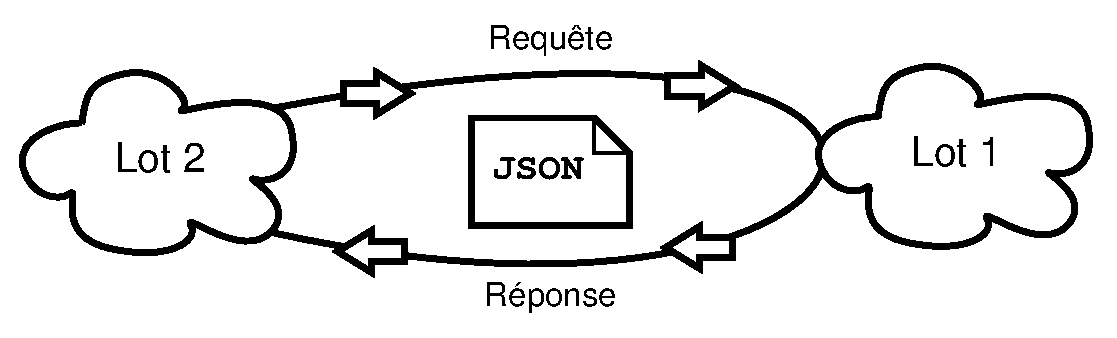
\includegraphics[scale=0.6]{eyrolles_webservices_echange}
	\caption{Principe de communication via \aws\ entre le \alotun\ et le \alotdeux\ d'\aey}
	\label{figure:eyrolles_webservices_echange}
\end{figure}

Les \awss\ à développer sur le \alotdeux\ sont les suivants :

\begin{itemize}
	\item le \aws\ des auteurs (initialisation et mise à jour) ;
	\item le \aws\ des collections (initialisation et mise à jour) ;
	\item le \aws\ des thématiques (initialisation) ;
	\item le \aws\ de demande de référencement ;
	\item le \aws\ de mise à jour des statuts de projets ;
	\item le \aws\ de mise à jour des informations commerciales des projets.
\end{itemize}

Tous ces types de \aws\ diffèrent en fait par l'adresse à laquelle ils doivent envoyer leur requête et par les paramètres qu'ils doivent fournir. Le processus d'échange de données avec le \alotun, quant à lui, est commun à tous. Le système à implémenter doit donc être modélisé, afin d'éviter d'écrire du code redondant et de faciliter une maintenance ultérieure. Cette étape de modélisation est une tâche clé du travail d'ingénieur, dans le sens où elle est nécessaire pour anticiper une évolution pérenne d'un système.

Le diagramme \auml\ de la figure~\ref{figure:eyrolles_webservices_uml} reprend la modélisation qui a été effectivement choisie.

\begin{figure}
	\centering
	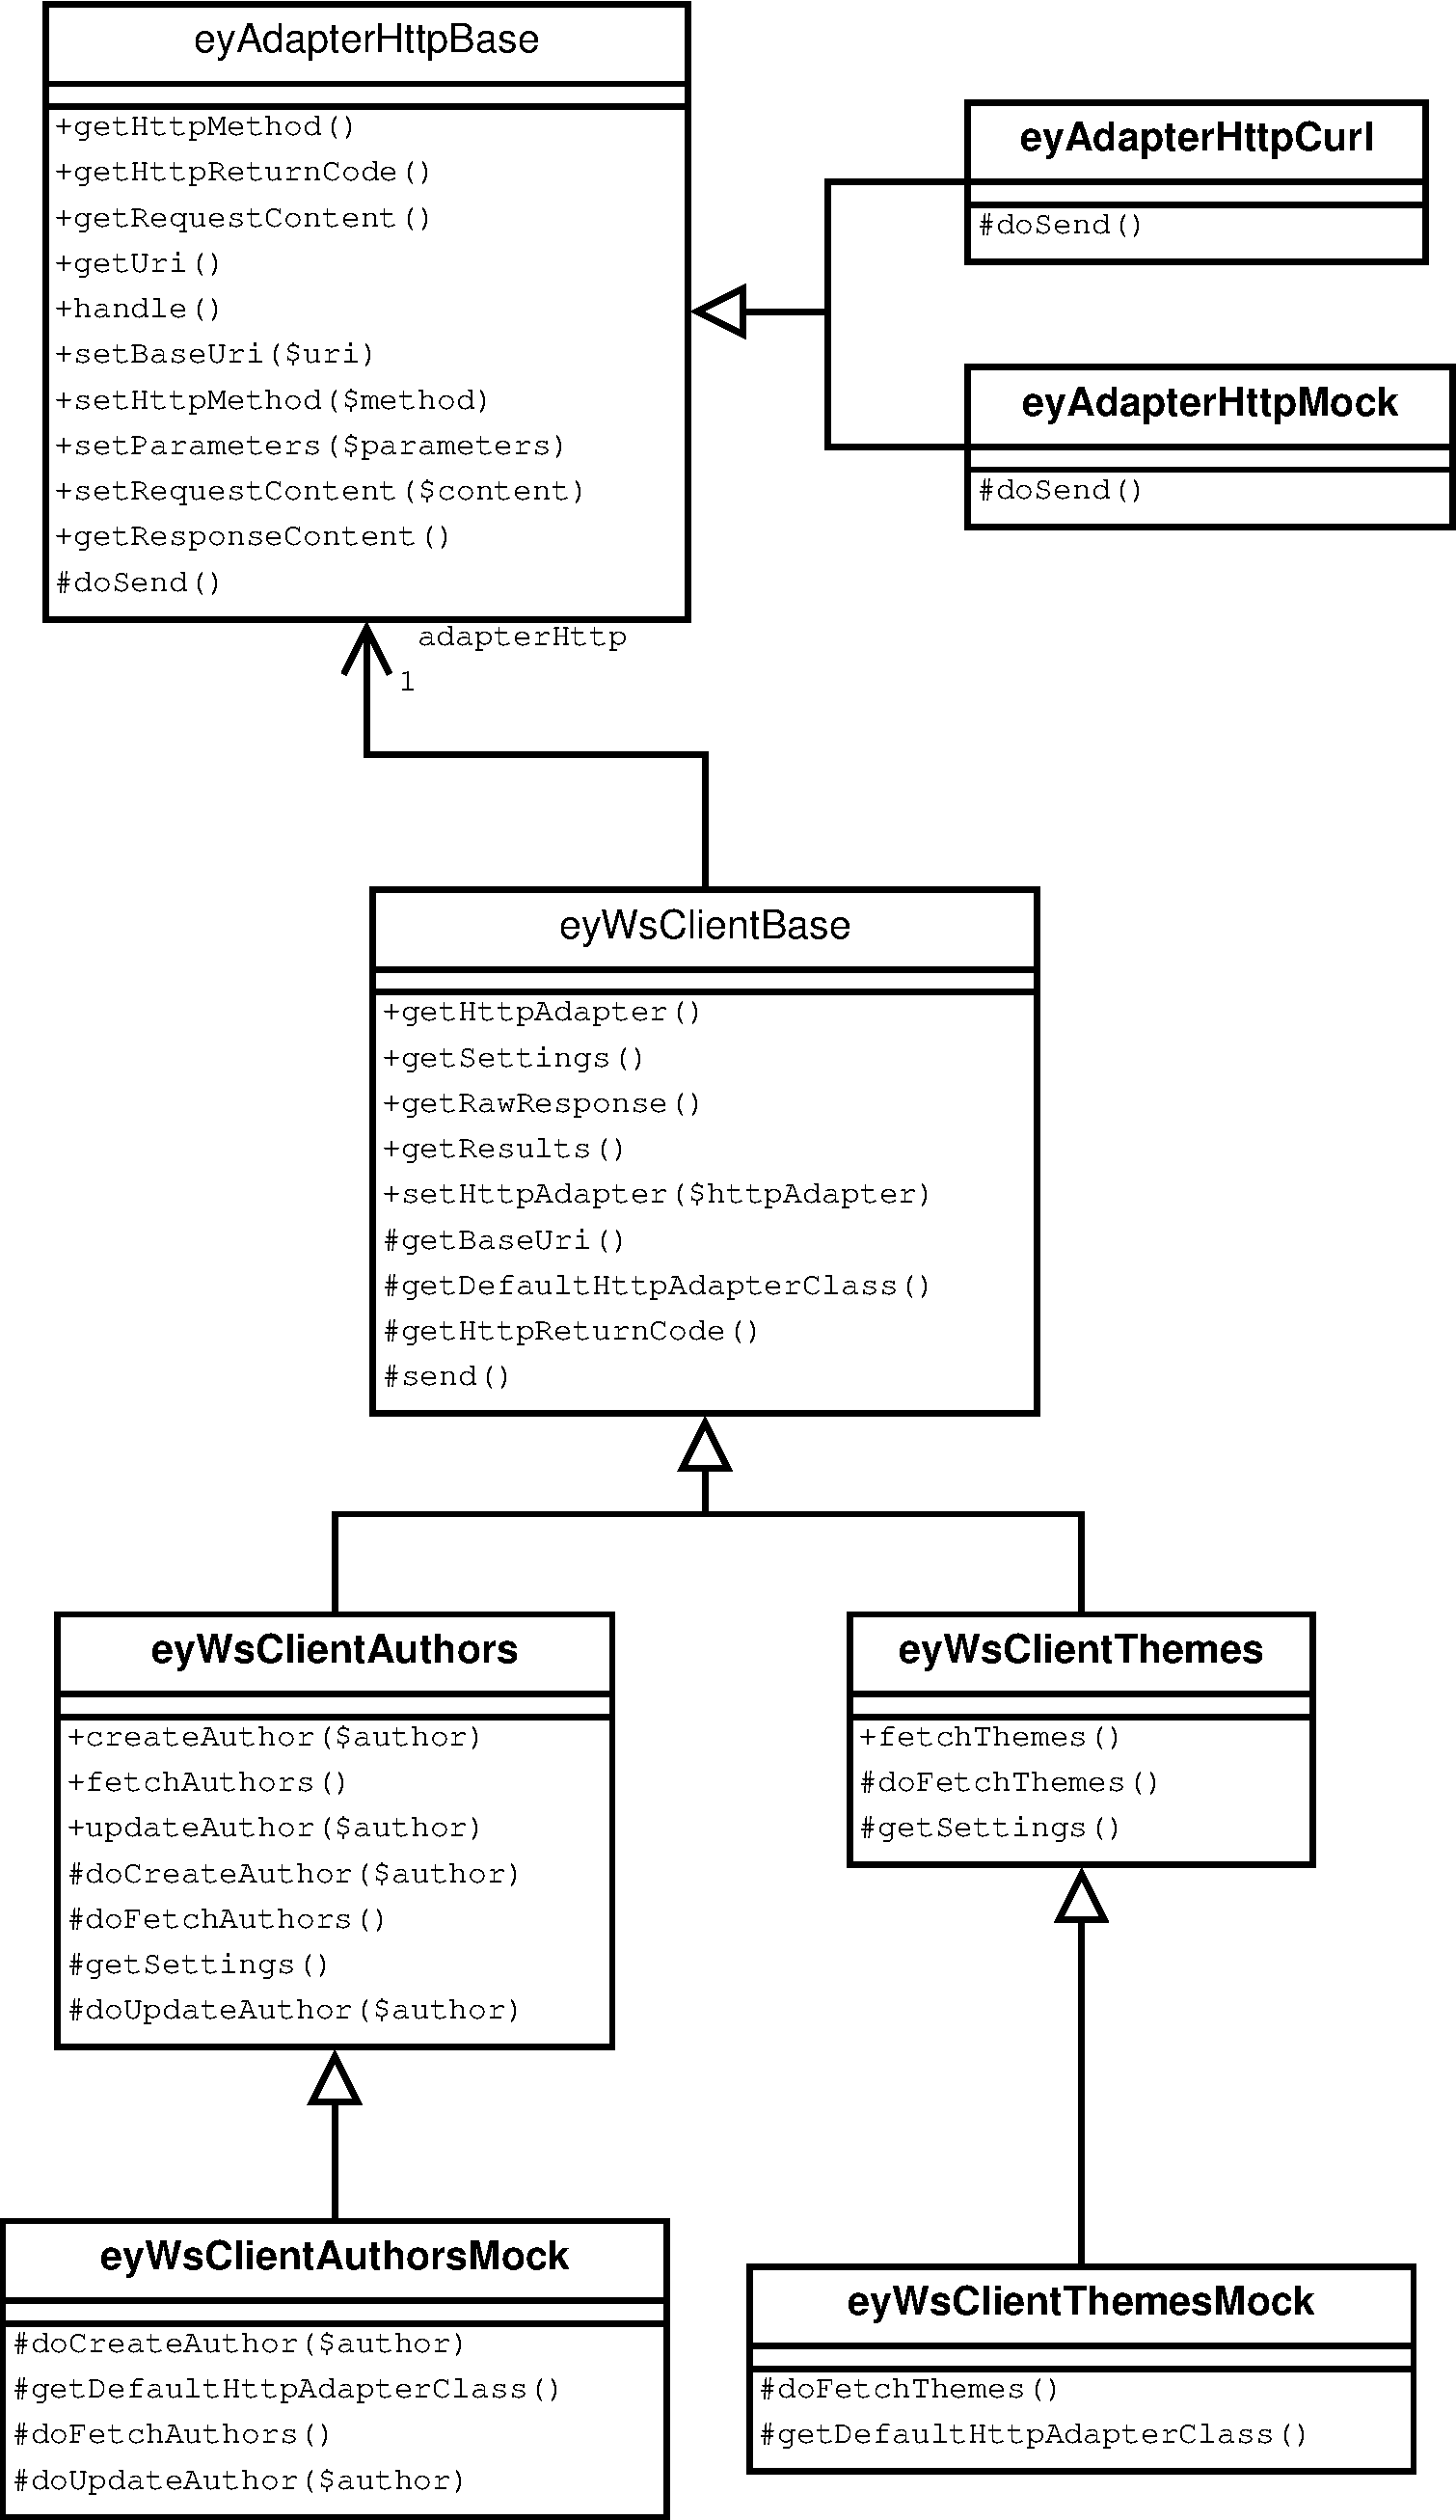
\includegraphics[scale=0.4]{eyrolles_webservices_uml}
	\caption{Modélisation des classes de \aws}
	\label{figure:eyrolles_webservices_uml}
\end{figure}

En effet, l'ensemble du code concernant la procédure de communication a été factorisé dans une classe \texttt{eyWsClientBase}. Les classes qui héritent de celle-ci, comme \texttt{eyWsClientAuthors} ou \texttt{eyWsClientThemes}, représentent les différents types de \aws. Au final, ces classes filles ne contiennent que les méthodes consistant à définir quels paramètres doivent être envoyés dans la requête, ou encore comment retourner la réponse à l'application.

Par ailleurs, l'implémentation de la liaison \ahttp\ a été isolée des classes de \aws\ : la classe abstraite \texttt{eyAdapterHttpBase} regroupe l'ensemble des méthodes permettant de stocker la méthode \ahttp\ à utiliser, les paramètres à envoyer ou encore l'adresse distante à consulter. Le contact effectif du \aws\ distant s'effectue dans la méthode \texttt{doSend()} surchargée dans les classes filles, telles que \texttt{eyAdapterHttpCurl} par exemple. Chaque classe \texttt{eyWsClient*} fait alors appel à une classe \texttt{eyAdapterHttp*} qui va se charger d'envoyer les données via le protocole \ahttp.

L'intérêt d'avoir différentes classes héritant de \texttt{eyAdapterHttpBase} permet de pouvoir implémenter de différentes façons l'appel au \aws\ distant. En effet, sur \aey, ce sont les fonctions de l'extension \acurl\footnote{La libraire \acurl\ donne la possibilité de récupérer, de créer ou encore de modifier le contenu d'une ressource accessible par le réseau, et supporte nottamment le protocole \ahttp.} de \aphp\ qui sont utilisées. En imaginant que l'\aintranet\ d'\aey\ soit déplacé sur un serveur sur lequel l'extension n'est pas installée, il serait très facile de réécrire une classe alternative, comme \texttt{eyAdapterHttpStream} qui utiliserait les fonctions \texttt{stream} disponibles en natif.

En outre, quand un développeur teste l'application du \alotdeux\ avec des données factices, il n'est pas concevable que celles-ci soient effectivement envoyées au \alotun\ pour le mettre à jour, au risque de corrompre l'intégrité des données de production. Il est donc nécessaire de prévoir une façon de simuler l'appel à un \aws.

Par exemple, dans le cas du \aws\ des auteurs, une classe \texttt{ey\-Ws\-Client\-Authors\-Mock} hérite de la classe \texttt{eyWsClientAuthors}. Entre autres, elle redéfinit la méthode sensée envoyer une requête de mise à jour d'un auteur au \alotun\ et ne fait rien à la place. Il est ainsi aisé de redéfinir des comportements initiaux, une fois que le problème a été modélisé en faisant appel aux grands principes de la programmation orientée objet.
